\chapter[Materiais e métodos]{Materiais e Métodos}

A análise do sistema foi feita de forma quantitativa por meio de estudo experimental em que foi realizada a montagem de um aparato experimental e a coleta de dados deste experimento visando analisar o consumo do motor com três diferentes configurações, sendo elas: motor operando somente com gasolina, motor acoplado a um gaseificador operando a topo aberto e a topo fechado, bem como a análise energética do sistema dada pela energia térmica do gás de síntese que pode ser convertida em trabalho de eixo ou energia elétrica.

\section{Aparato experimental}
Para a alimentação do motor com o gás de síntese proveniente da gaseificação do bagaço de cana, foi montado um aparato experimental composto por um reator, um sistema de resfriamento dos gases e um motor de combustão interna na configuração do gaseificador a topo aberto. A topo fechado, foi adicionado ao aparato um compressor a montante do reator.

O reator utilizado, visto na Figura \ref{foto_reator}, possui 125mm de diâmetro e 500mm de altura. Antes de sua utilização, foram realizadas soldas no seu corpo externo para reparo do material, que tinha fundido. Adicionou-se argamassa refratária na parte interna para evitar transferência de calor com o meio, reduzindo seu diâmetro interno de 150mm para 125mm. O isolamento térmico foi feito com lã de vidro e manta térmica envoltos por uma cinta térmica.

\begin{figure}[!htb]
	\centering
	\subfloat[a]{
		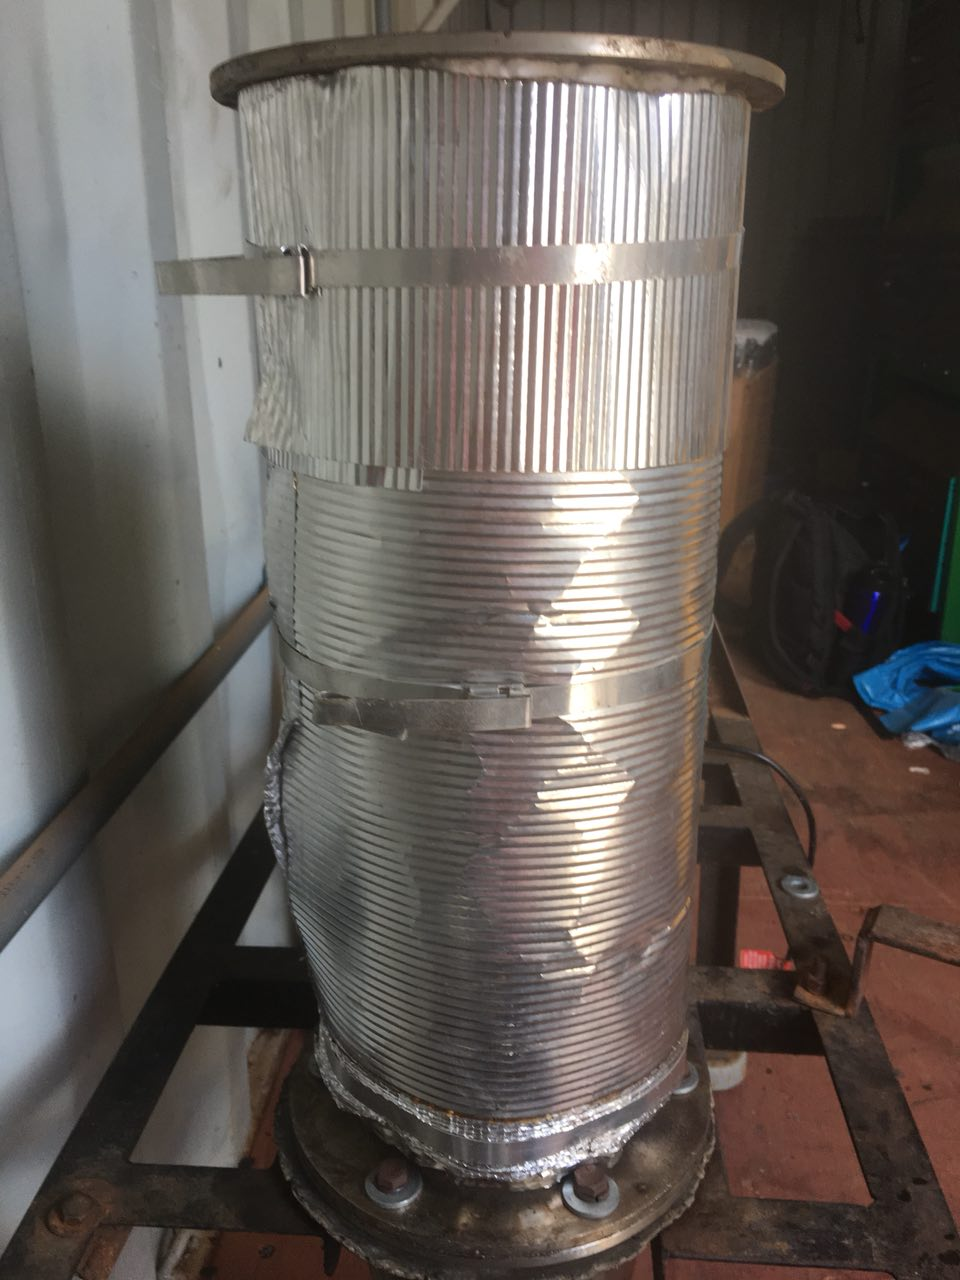
\includegraphics[width=5.5cm]{Figuras/reator}
	}
	\quad %espaco separador
	\subfloat[b]{
		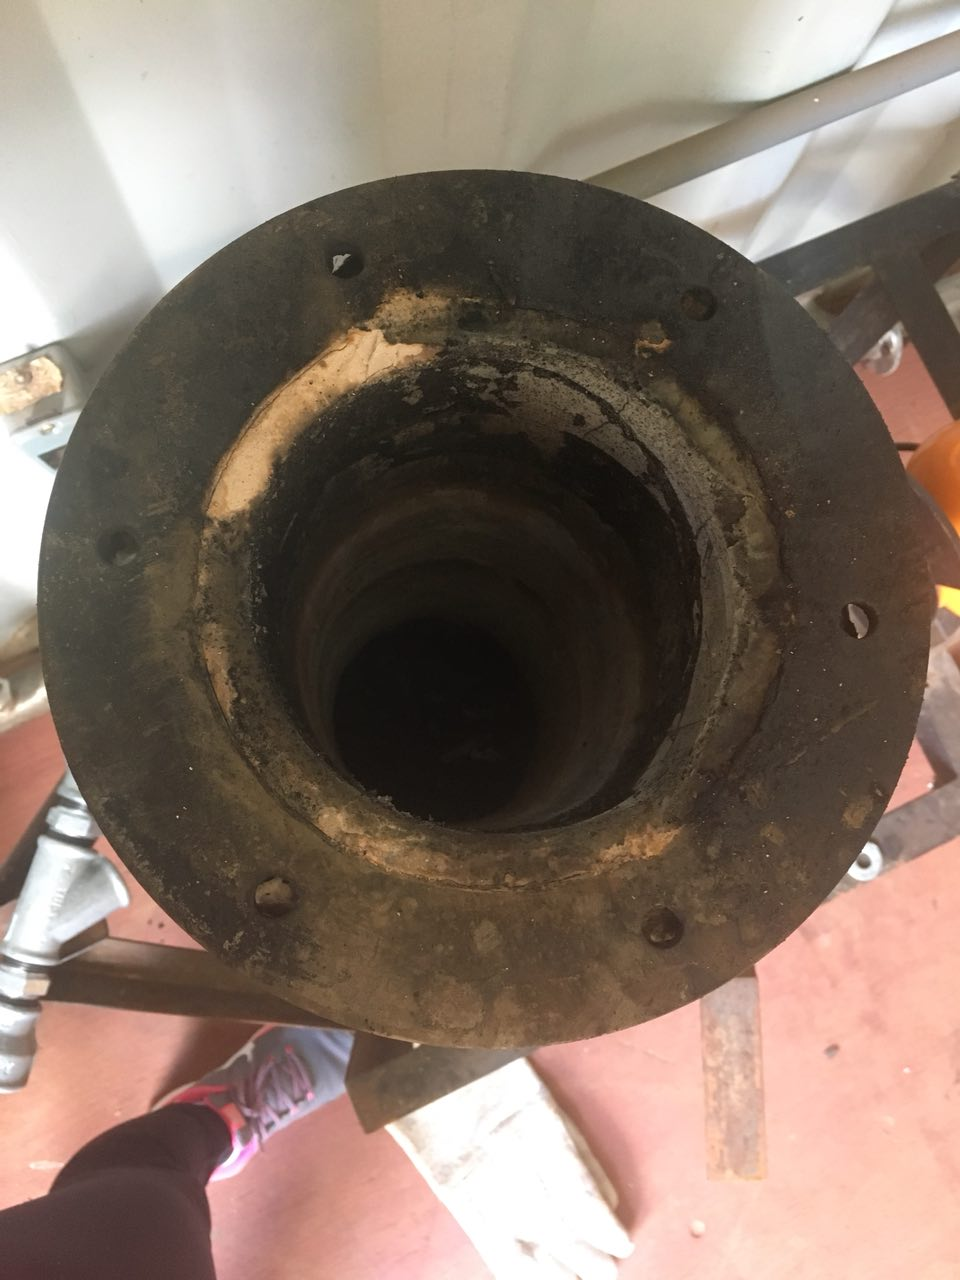
\includegraphics[width=5.5cm]{Figuras/reator_cima}
	}
	\caption{Reator (Fonte: autoria própria).}
	\label{foto_reator}
\end{figure}

Na saída do reator foi colocada uma mangueira que era resfriada em água à temperatura ambiente dentro de um galão de plástico. A água, além de resfriar o gás, condensou o alcatrão presente nele, este alcatrão se depositou nas paredes da própria mangueira. Este sistema e a mangueira com o alcatrão condensado podem ser vistos na Figura \ref{sistema_limpeza}.

\begin{figure}[!htb]
	\centering
	\subfloat[a]{
		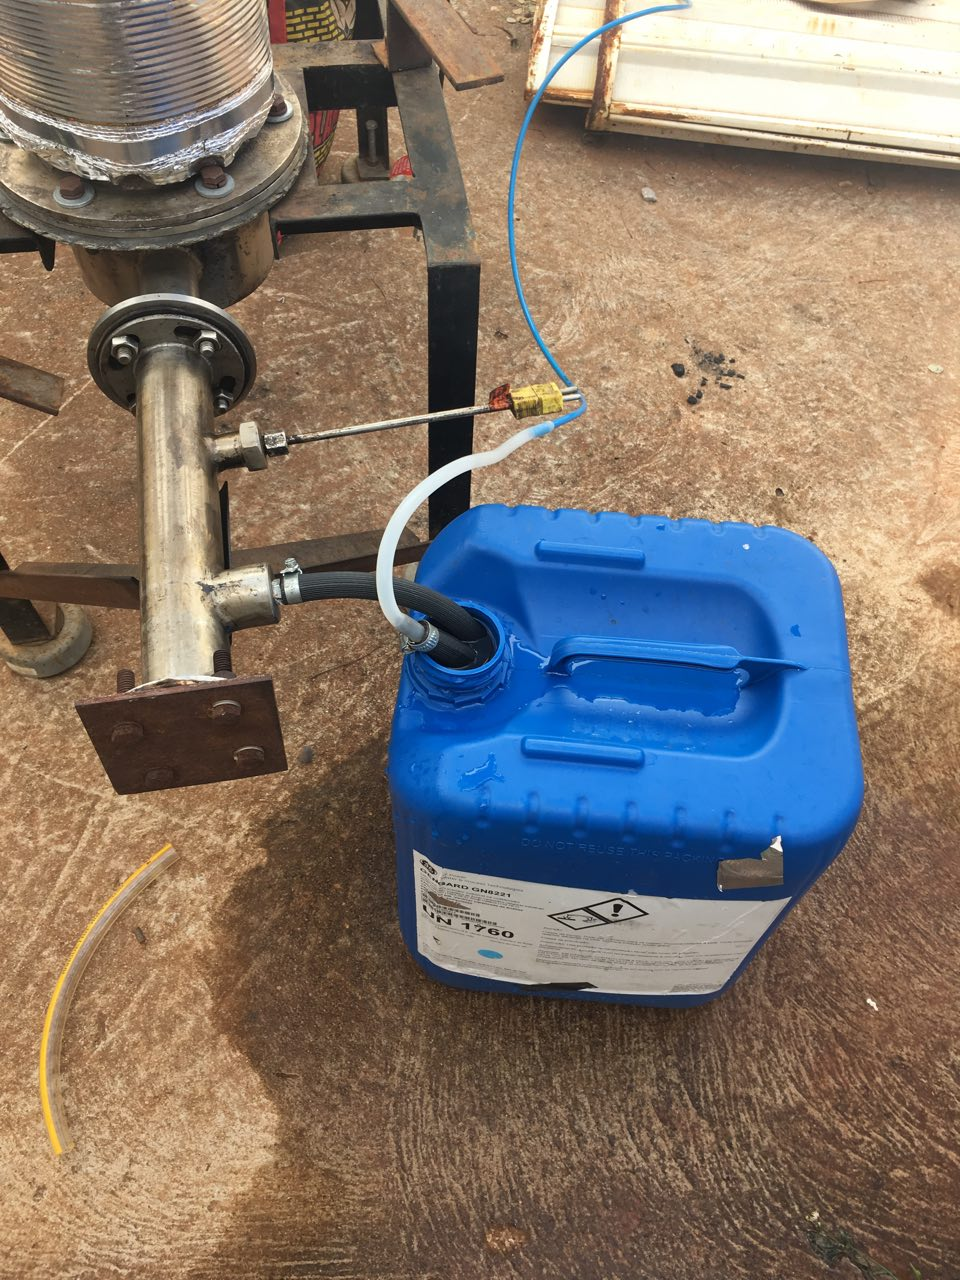
\includegraphics[width=5cm]{Figuras/sistema_limpeza}
	}
	\quad %espaco separador
	\subfloat[b]{
		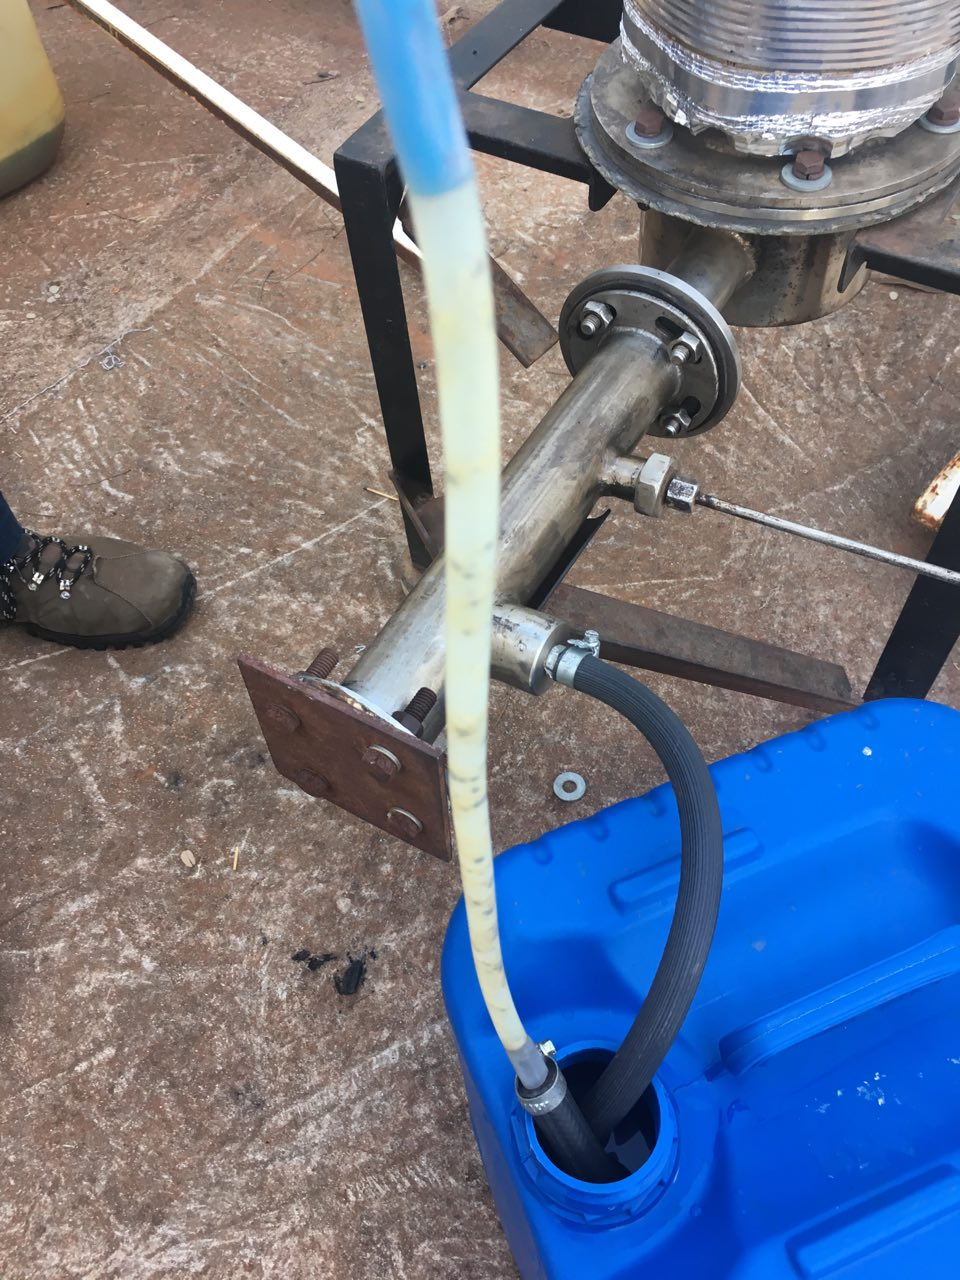
\includegraphics[width=5cm]{Figuras/alcatrao_condensado}
	}
	\caption{a) Resfriamento do gás e condensação do alcatrão. b) Alcatrão condensado. (Fonte: autoria própria).}
	\label{sistema_limpeza}
\end{figure}

O fluxo de gás seguiu por outra mangueira até a entrada de ar do motor, que na Figura \ref{entrada_gas}, é a mangueira azul. O motor utilizado foi um motor de combustão interna de um Fiat Palio 1.0 8V.

\begin{figure}[!htb]
	\centering
	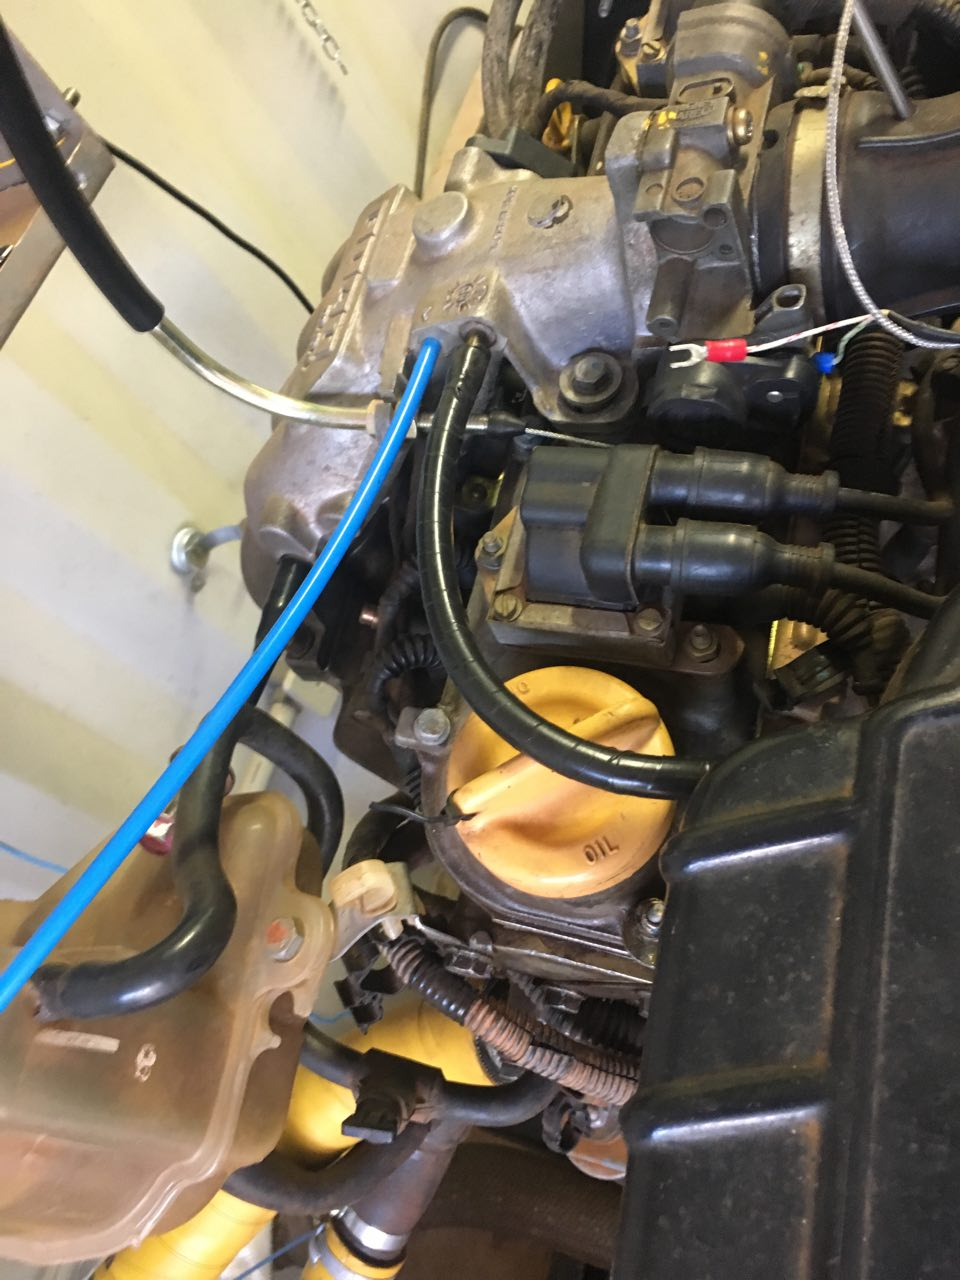
\includegraphics[width = 5cm]{Figuras/entrada_gas}
	\caption{Entrada do gás de síntese no motor. (Fonte: autoria própria)}
	\label{entrada_gas}
\end{figure}

Para que o reator trabalhasse em modo downdraft, o ar era puxado pelo vácuo do motor, dessa forma, causava-se uma depressão na saída do reator, fazendo com que o ar fosse puxado do topo, passasse pelo corpo deste servindo como agente oxidante das reações, e produzindo gás de síntese, que seguia o fluxo até o motor.

\section{Procedimento Experimental}

Para preparar a biomassa para o experimento de gaseificação, cortou-se o bagaço de cana em pedaços, como mostra a Figura \ref{bagaco_cortado}, e este foi deixado secando ao sol por mais de 30 dias. Separou-se, então, os bagaços em diferentes sacolas, cada uma com 100g, que foram pesadas com uma balança digital portátil.

\begin{figure}[!htb]
	\centering
	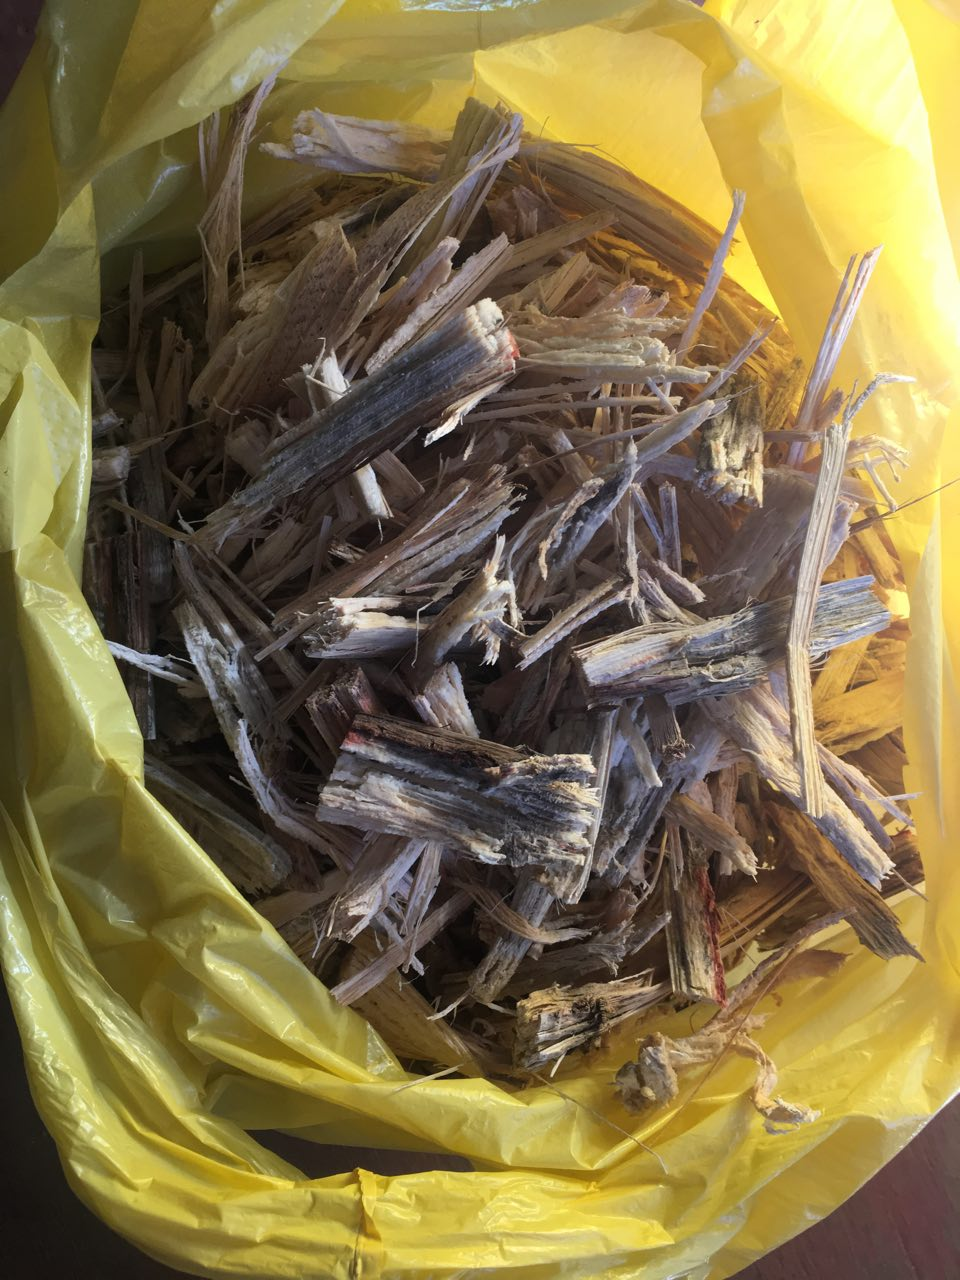
\includegraphics[width=6cm]{Figuras/bagaco_cortado}
	\caption{Biomassa preparada para gaseificação. (Fonte: autoria própria)}
	\label{bagaco_cortado}
\end{figure}

O experimento iniciou com a coleta de dados do motor funcionando apenas com gasolina através do software **. Foram coletados dados da rotação do motor, o tempo de injeção, a posição da borboleta e a pressão do coletor, dentre outros dados fornecidos pelo software.

Após coletados esses dados, deu-se ínio ao processo de gaseificação no reator com a adição, primeiramente, de carvão para dar ignição até que se atingisse a temperatura de gaseificação e entrasse em regime permanente.
A partir de então, adicionavam-se 100 gramas de bagaço de cana medindo a altura da coluna no reator ocupada por ele e o tempo levado até que todo o bagaço inserido fosse consumido e transformado em gás de síntese. A alimentação do bagaço de cana foi realizada manualmente pelo topo do reator e foi feita até que fossem coletados os dados do motor operando a duplo combustível.

Depois de coletados os dados a topo aberto, adicionou-se 200g de biomassa, fechou-se o topo do reator pressurizando-o, e injetou-se ar com um compressor até que fossem coletados os dados do software e da vazão volumétrica do ar com um rotâmetro.

\section{Consumo do motor}

O cálculo do consumo de combustível do motor pode ser feito pela equação \ref{eq:consumo}.

\begin{equation} \label{eq:consumo}
	C = \dot{Q} * t\textsubscript{i} * N * {2 \pi*60} \qquad [L/h]
\end{equation}

Onde C é o consumo,
$\dot{Q}$ é a vazão volumétrica do bico de injeção do motor,
t\textsubscript{i} é o tempo de injeção e
N é a rotação do motor.

\section{Análise energética teórica}
\subsection{Poder Calorífico do gás de síntese}

De acordo com a metodologia de \cite{tiangco1986}, o poder calorífico do gás pode ser obtido através da equação \ref{PCI_Tiangco}.

\begin{equation} \label{PCI_Tiangco}
	PCI\textsubscript{gás} = 5,9417 - 8,2893*10\textsuperscript{-3} * \psi \qquad [MJ/Nm^3]
\end{equation}

Onde $\psi$ é a taxa específica de processamento de um reator, que pode ser obtida pela equação \ref{taxa_reator}, e está compreendida entre os valores de 100 a 400 kg/m$^2$h.

\begin{equation} \label{taxa_reator}
	\psi = \frac{\dot{m}\textsubscript{biomassa}}{A\textsubscript{g}} \qquad [\frac{kg}{m^2*h}]
\end{equation}

Onde $\dot{m}$\textsubscript{biomassa} é a vazão da biomassa, que pode ser obtida pela equação \ref{vazao_biomassa_PCI} e A\textsubscript{g} é a área da seção transversal do gaseificador.

\begin{equation} \label{vazao_biomassa_PCI}
\dot{m}\textsubscript{biomassa} = \frac{A\textsubscript{g} * h_b * \rho\textsubscript{ap}}{t} \qquad [kg/h]
\end{equation}

Onde
h$_b$ é a altura do leito consumido,
$\rho$\textsubscript{ap} é a massa específica aparente do bagaço de cana medida com a massa de bagaço consumida pelo volume ocupado no reator e
t é o tempo de consumo da biomassa.

\subsection{Vazão do gás de síntese}

Para determinação da vazão do gás de síntese, faz-se um balanço de energia, de acordo com a equação \ref{balanco_massa}.

\begin{equation}\label{balanco_massa}
	\dot{Q}\textsubscript{bagaço} + \dot{Q}\textsubscript{ar} = \dot{Q}\textsubscript{syngas}\qquad [m^3/h]
\end{equation}

onde $\dot{Q}$\textsubscript{bagaço} pode ser dado pela vazão mássica do bagaço vezes sua massa específica aparente.

\begin{equation} \label{qdot_bagaco}
	\dot{Q}\textsubscript{bagaço} = \dot{m}\textsubscript{bagaço} * \rho\textsubscript{ap} \qquad [m^3/h]
\end{equation}

\subsection{Vazão mássica do bagaço de cana}

A vazão mássica do bagaço é determinada pela massa de biomassa inserida pelo tempo que foi consumida e pode ser calculada pela equação \ref{vazao_bagaco}.

\begin{equation} \label{vazao_bagaco}
\dot{m}\textsubscript{bagaço} = \frac{m\textsubscript{bagaço}}{t} \qquad [m/s]
\end{equation}

\subsection{Potência térmica}

A potência do gás pode ser calculado pela equação \ref{consumo energetico}, que será caluclada com o PCI da metodologia de Tiangco.

\begin{equation} \label{consumo_energetico}
\dot{E} = \dot{Q} * PCI   \quad\quad  [J/s]
\end{equation}

Portanto, a equação \ref{potencia_termica} dá a potência térmica do gás de síntese do bagaço, que pode ser transformado em trabalho de eixo.

\begin{equation} \label{potencia_termica}
P\textsubscript{t} = \dot{Q}\textsubscript{syngas} * PCI\textsubscript{syngas} \quad\quad  [W]
\end{equation}

\subsection{Eficiência}

A eficiência energética de um motor a combustão leva em conta diversas perdas na conversão da energia, tais como a transferência de calor para as paredes da câmara,
a energia mecânica de expansão dos gases nos cilindros, a conversão da energia térmica do combustível em trabalho mecânico, dentre outros. A eficiência total para um motor a combustão, portanto, pode ser calculada pela equação \ref{eficiencia_motor}, onde $\eta$\textsubscript{c} é a eficiência de combustão, $\eta$\textsubscript{a} é a eficiência adiabática, $\eta$\textsubscript{t} é a eficiência térmica, $\eta$\textsubscript{p} é a eficiência de propriedade dos fluidos, $\eta$\textsubscript{i} é a eficiência inerente, e$_b$ é a eficiência de bombagem e $\eta$\textsubscript{m} é a eficiência mecânica \cite{martins2006}.

\begin{equation} \label{eficiencia_motor}
\eta\textsubscript{motor} = \eta\textsubscript{c} * \eta\textsubscript{a} * \eta\textsubscript{t} * \eta\textsubscript{p} * \eta\textsubscript{i} * e_b \eta\textsubscript{m} 
\end{equation}

Para um moto-gerador, além das eficiências supracitadas, consideram-se as perdas na conversão da energia mecânica em energia elétrica no gerador, dada pela eficiência do gerador $\eta$\textsubscript{g}. A eficiência total para um moto-gerador pode ser calculada pela equação \ref{eficiencia_gerador}

\begin{equation} \label{eficiencia_gerador}
\eta\textsubscript{moto-gerador} = \eta\textsubscript{motor} * \eta\textsubscript{g}
\end{equation}


\subsection{Potência de eixo e Potência elétrica}

A eficiência da conversão energética de uma máquina pode ser dada pela razão da potência ou energia que foi gerada sobre a potência ou energia de entrada. Portanto, para um motor e um moto-gerador, as potência de eixo e elétrica podem ser calculadas pelas equações \ref{potencia_eixo} e \ref{potencia_eletrica}, respectivamente.

\begin{equation} \label{potencia_eixo}
P\textsubscript{w} = P\textsubscript{t} * \eta\textsubscript{motor} \qquad [W]
\end{equation}

\begin{equation} \label{potencia_eletrica}
P\textsubscript{e} = P\textsubscript{t} * \eta\textsubscript{moto-gerador} \qquad [W]
\end{equation}


